\documentclass[a4paper, oneside]{book}
% Note the preamble is imported, from /semester/topic
% Basic packages
\usepackage[T1]{fontenc}
\usepackage[utf8]{inputenc}
\usepackage{babel}
\usepackage[square]{natbib}
\usepackage{hyperref}
\usepackage{xpatch}
\usepackage{enumerate}
\usepackage{todonotes}
\usepackage{tcolorbox}
\usepackage{framed}
\usepackage{blindtext}
\usepackage{color}
\usepackage{titlesec}

% Math Packages
\usepackage{mathtools}
\usepackage{amssymb}
\usepackage{amsthm}
\usepackage{bbm}
\usepackage{bm}
\usepackage{amsmath}

\usepackage{xifthen}

% ENVIRONMENTS & THEIR CONFIGURATIONS
\renewcommand{\qedsymbol}{$\blacksquare$} % Use a black box to end proofs

% Custom environments
\theoremstyle{plain}
\newtheorem{theorem}{Theorem}[chapter]
\newtheorem{lemma}[theorem]{Lemma}
\newtheorem{proposition}[theorem]{Proposition}
\newtheorem{corollary}[theorem]{Corollary}
\newtheorem{exercise}[theorem]{Exercise}

\theoremstyle{definition}
\newtheorem{DEFN}[theorem]{Definition}
\newtheorem{EXMP}[theorem]{Example}
\newenvironment{definition}{\begin{leftbar}\begin{DEFN}}{\end{DEFN}\end{leftbar}}
\newenvironment{example}{\begin{EXMP}}{\hfill$\square$\end{EXMP}}

\theoremstyle{remark}
\newtheorem{remark}{Remark}
\newtheorem{note}{Note}

% Chance apperenace of chapters
\definecolor{gray75}{gray}{0.75}
\titleformat{\chapter}[hang]{\Huge\bfseries}{\thechapter\hspace{5pt}| \hspace{10pt}}{0pt}{\Huge\bfseries}

% Basic notations
\newcommand{\N}{\mathbb{N}}
\newcommand{\Z}{\mathbb{Z}}
\newcommand{\Q}{\mathbb{Q}}
\newcommand{\F}{\mathbb{F}}
\newcommand{\R}{\mathbb{R}}
\newcommand{\C}{\mathbb{C}}
\newcommand{\e}{\mathrm{e}}

% shorthands & special notations
\newcommand{\Range}{\text{range}}
\newcommand{\Span}{\text{span}}
\newcommand{\Null}{\text{null}}
\newcommand{\Ker}{\text{ker}}
\newcommand{\ind}{\mathbbm{1}}
\newcommand{\bigO}{\mathcal{O}}
\newcommand{\mb}[1]{\mathbf{#1}}

\newcommand{\norm}[1]{\lvert\lvert#1\rvert\rvert}
\newcommand{\abs}[1]{\lvert#1\rvert}

% Command for lectures
\makeatother
\def\@lecture{}%
\newcommand{\lecture}[3]{
    \ifthenelse{\isempty{#3}}{%
        \def\@lecture{Lecture #1}%
    }{%
        \def\@lecture{Lecture #1: #3}%
    }%
    \chapter*{\@lecture}
    \textbf{Date}: #2 \\
}
\makeatletter


\author{Martin Sig Nørbjerg}


\title{Ansøgning til studie job}

\begin{document}
\maketitle

\chapter*{Ansøgning, hjælpelærer i matematik (2022)}
Hej,
\\ \\
Jeg er en frisk, 20 årig, 4. semesters (5. semester til 1. sebtember) matematik studerende, som godt kunne tænke sig et studierelavant studiejob. Jeg ser jobbet som en fantastisk mulighed for at forbedre mine egne færdigheder i forhold til at lære fra mig. Samtidigt tror jeg at jobbet som hjælpelærer, kunne være utroligt tilfredsstillende.
Jeg elsker følelsen af succes når det slår klik og brikkerne falder på plads for mig og mine medstuderende, efter at have sparret sammen en opgave eller et resultat vi ikke helt forstår.
\\ \\
Håber at jeg kan blive taget i betragtning, personligt vil jeg helst være hjælpelærer i følgende fag og i oplistede rækkefølge:
\begin{enumerate}
    \item \textit{Programmering for matematikere:} Da jeg både før og igennem min studietid har brugt meget af min fritid på at programmere, som en slags hobby, (dog kan jeg ikke huske om dette er noget man har på første semester eller andet semester).
    \item \textit{Calculus / Lineær algebra:} Tror jeg ville egne mig bedst som Calculus hjælpelærer, såfremt ``programmering for matematikere'' ikke er en mulighed, dog vil jeg foretrække lineær algebra, da jeg finder dette mere intressant.
\end{enumerate}

\subsection*{Kontaktoplysninger}
\textit{Navn}: Martin Sig Nørbjerg \\
\textit{Telefon}: (+45) 51 15 09 93 \\
\textit{Email}: mnarbj20@student.aau.dk \\
\textit{Adresse}: Grønnegade 2, st tv, 9000 Aalborg

\chapter*{CV}

\subsection*{Education}
\begin{enumerate}
      \item \textbf{Mathematics}, Aalborg University - Bachelor\\
        \textit{Sebtember 2020 - Today}\\
        Currently, I'm persuing bachellor in applied mathematics from Aalborg university. Where we mostly work in groups either with the general study of mathematics or with larger projects.

      \item \textbf{HTX (Global Technology)}, Herningsholm - Gymnasiel uddandelse\\
        \textit{August 2017 - June 2020}\\
        At Herningsholm most of the classes were split between the classics like science and humanities as well as group projects with a focus on product development.

\end{enumerate}

% \subsection*{Projects that i'm proud of}
% \begin{enumerate}[i)]
%   \item \textbf{Herb} - Neural Networks and Reinforcement Learning.
%         An implementation of Google Deepminds Alpha Zero Algorithm, on the game of go (using a 9x9 board, instead of a 19x19), built with Python, PyTorch, Numpy and the performance-critcal code was JIT-compiled with the Numba liberary
%     \textit{Github repository:} % TODO
% \end{enumerate}


\subsection*{Previous Work Experience}
\begin{enumerate}
      \item \textbf{Fakta}, Ikast - Key Carrier\\
        \textit{Sebtember 2019 - April 2020}\\
        Was in charge of the store during shits, including the supervission of younger service employees and the closing of the store.

      \item \textbf{Fakta}, Ikast - Service Employee\\
        \textit{May 2017 - Sebtember 2019}\\
        Primairly working as a cashier, secondarly working on keeping the store presentable.


\end{enumerate}
\subsection*{Skills}
\begin{itemize}
  \item Programming (Python, a bit of Rust, R, and a tiny bit of machine learning).
  \item Mathematics (Or atleast every thing up until 4. semester ;)).
\end{itemize}

\chapter*{Studie journal}
\begin{figure}[h]
  \centering
  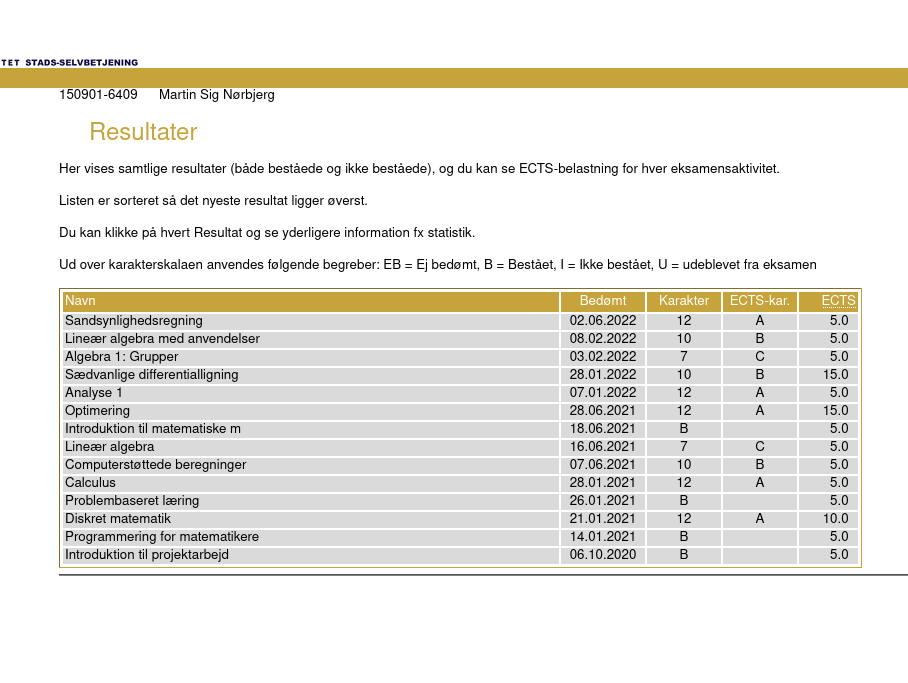
\includegraphics[scale=0.5]{studie_journal.png}
\end{figure}


\end{document}
